\section{Opis wykorzystanych technologii i narzędzi}


\subsection{Kody graficzne QR}
Przedstawianie danych w postaci kodów graficznych nie jest niczym innowacyjnym. Towary w sklepach od dawna oznaczane są za pomocą jednowymiarowego kodu kreskowego. Kombinacja jasnych oraz ciemnych linii umożliwia przechowywanie danych, które odczytywane są za pomocą skanera z laserem. Tego typu metody stosuje się głównie w celach identyfikacji. Do przechowywania większej ilości danych wykorzystuje się częściej tzw. kody 2D.
 
\begin{wrapfigure}[10]{r}{0.25\textwidth}
	\vspace{-15pt}
	\begin{center}
		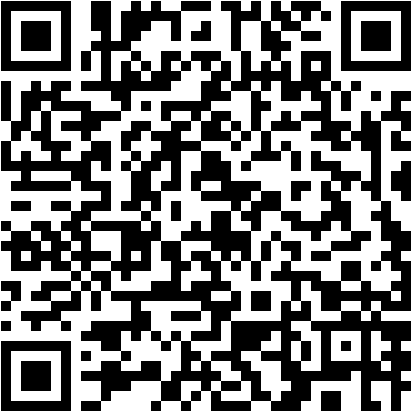
\includegraphics[width=0.25\textwidth]{02/qr_title}
	\end{center}
	\vspace{-10pt}
	\caption{Tytuł pracy przedstawiony w postaci kodu QR}
	\vspace{-10pt}
\end{wrapfigure}

Kody QR (ang. Quick Respone - szybka odpowiedź) to dwuwymiarowe, matrycowe, kwadratowe kody graficzne. Składają się z modułów, czyli kombinacji ciemnych oraz jasnych kwadratów, które są nośnikami danych. Zostały stworzone przez japońską firmę Denso-Wave w 1994 r \cite{thonky_tutorial}. Według postanowień licencyjnych mogą być wykorzystywane bez żadnych opłat, a sam standard jest opisany w normie ISO/IEC 18004:2015 \cite{norma_qr}. Dzięki dodatkowemu wymiarowi, pozwalają na przechowywanie większej ilości informacji (do ok. 7000 liczb lub 4000 znaków alfanumerycznych) niż kody kreskowe, posiadające tylko jeden wymiar. Ponadto, zapewniają zdecydowanie lepszą korekcję błędów. Nawet częściowo uszkodzony kod może zostać poprawnie odczytany. Posiadają kilka miejsc szczególnych do ułatwienia orientacji podczas odkodowywania. Ich liczba zależy od rozmiaru kodu.

Pierwotnie bardzo duże zastosowanie kody QR znalazły w logistyce, gdzie zawierały informacje o przesyłanych paczkach. Współcześnie kojarzone są przeważnie z urządzeniami mobilnymi. Spotykane na przystankach, w sklepach lub magazynach służą do komunikacji z użytkownikami smartfonów, przełamując niejako barierę między światem wirtualnym, a rzeczywistym. Kod zawiera informacje w postaci liczb, liter i symboli. Jednak odpowiednie formatowanie informacji, pozwala na dodatkowe interpretowanie ich przez urządzenie przenośne. I tak po zeskanowaniu może zostać wysłana wiadomość e-mail, albo dodany numer do kontaktów. Najczęściej jednak zawierają adresy URL, które powodują wyświetlenie odpowiedniej strony w przeglądarce internetowej telefonu.

% jeszcze można zrobić część o budowie kodu, gdzie wstawi się grafikę z wiki i opowie o tym z jakich elementów się składa
\subsubsection*{Sposoby kodowania, generowani oraz odczytywania}
Przedstawiając informacje w postaci kodu QR trzeba najpierw określić rodzaj oraz ilość danych, jakie mają zostać zakodowane. Istnieją trzy główne parametry: wersja, rodzaj danych oraz poziom korekcji błędów.

Wersje to inaczej rozmiary kodu numerowane od 1 do 40. Decydują o ilości modułów, czyli wielkości danych jakie można przechować. Wersja pierwsza posiada 21x21 modułów, każda kolejna jest większa o trzy na każdy bok i tak do 40, zawierającej 177x177 modułów. 

Rodzaj kodowanych danych zależny jest od typu informacji, jaka ma być przechowywana. Ten parametr wpływa na ilość bitów przypadającą na jeden znak, oraz na sposób w jaki dane mają zostać odkodowane.  Także wpływa na maksymalny rozmiar:
\begin{itemize}
	\item \textbf{Numeryczny} -- cyfry 0 - 9. Pozwala na zakodowanie do 7089 znaków.
	\item \textbf{Alfanumeryczny} -- oprócz cyfr, także pozwala na przechowywanie wielkich liter oraz znaków: '\$', '\%', '*', '+', '-', '.', '/', ':' i spację. Można zakodować do 4296 znaków. 
	\item \textbf{Binarny} -- domyślnie dla zestawu znaków z ISO-8859-1, pozwala też na UTF-8. Maksymalnie 2953 znaków.
	\item \textbf{Kanji} -- znaki z systemu kodowania Shift JIS. Do 1817 znaków.
\end{itemize}

Poziom korekcji błędów służy do określenia czy dane zostały odczytane poprawnie. Pozwala także na odzyskanie części danych, nawet jeśli kod został uszkodzony, dzięki algorytmowi Reeda-Solomona. Specyfikacja wyróżnia cztery poziomy korekcji. Obok każdego z nich podany został procent danych, jakie można odzyskać:
\begin{itemize}
	\item \textbf{L (Low)} - 7\% danych,
	\item \textbf{M (Medium)} - 15\% danych,
	\item \textbf{Q (Quartile)} - 25\% danych,
	\item \textbf{H (High)} - 30\% danych.
\end{itemize}

\begin{center}
	\begin{tabular}{| c | c | c | c | c | c | c |}
		\hline
		Wersja & Moduły & Korekcja & Numeryczny & Alfanumeryczny & Binarny & Kanji\\
		\hline
		\multirow{4}{*}{1} & \multirow{4}{*}{21x21}&L&41&25&17&10\\
		& & M&34&20&14&8\\
		& & Q&27&16&11&7\\
		& & H&17&10&7&4\\
		\hline
		\multirow{4}{*}{40} & \multirow{4}{*}{177x177}&L&7089&4296&2953&1817\\
		& & M&5596&3391&2331&1435\\
		& & Q&3993&2420&1663&1024\\
		& & H&3057&1852&1273&784\\
		\hline
	\end{tabular}
\end{center} 
Istnieje wiele sposobów na generowanie kodów QR. Jednym z nich są strony www, gdzie po podaniu danych i parametrów można pobrać kod w postaci obrazka. Innym rozwiązaniem jest skorzystanie z gotowych bibliotek i wygenerowanie takiego kodu z poziomu kodu. I na przykład w Pythonie można skorzystać z modułu \textit{qrcode}.

Odczytanie, czyli odkodowanie informacji także możliwe jest na wiele sposobów. Razem z systemami mobilnymi często dostarczane są wbudowane czytniki, wykorzystujące do tego celu wbudowaną kamerę. Podobnie, takie rozwiązanie możliwe jest dzięki odpowiednim biblioteką. W Androidzie jest to dostępna za darmo \textit{Zebra Crossing}.


\subsection{System Android}
\subsection{Aplikacja internetowa w Django}
